\section{Theory}
The Restricted Boltzmann Machine (RBM) is an energy-based model defined by the energy function
\begin{align}
    E(\vec{v}, \vec{h})
        &= -\sum_i a_i v_i - \sum_j b_j h_j - \sum_{i,j} v_i w_{ij} h_j \label{eq:rbm_energy} \\
        &= -\vec{a}^\intercal\vec{v} - \vec{b}^\intercal\vec{h} - \vec{v}^\intercal\mat{W}\vec{h} \label{eq:rbm_energy_vectorized}
\end{align}
where
\begin{itemize}
    \item \( \vec{v} \in \Z_2^{n_v} \) represents the visible units, with associated bias vector \( \vec{a} \in \R^{n_v} \).
    \item \( \vec{h} \in \Z_2^{n_h} \) represents the hidden units, with associated bias vector \( \vec{b} \in \R^{n_h} \).
    \item \( \mat{W} \in \R^{n_v \times n_h} \) represents the weights corresponding to the interaction strengths between visible and hidden units.
\end{itemize}

\begin{figure}[ht]
    \begin{center}
        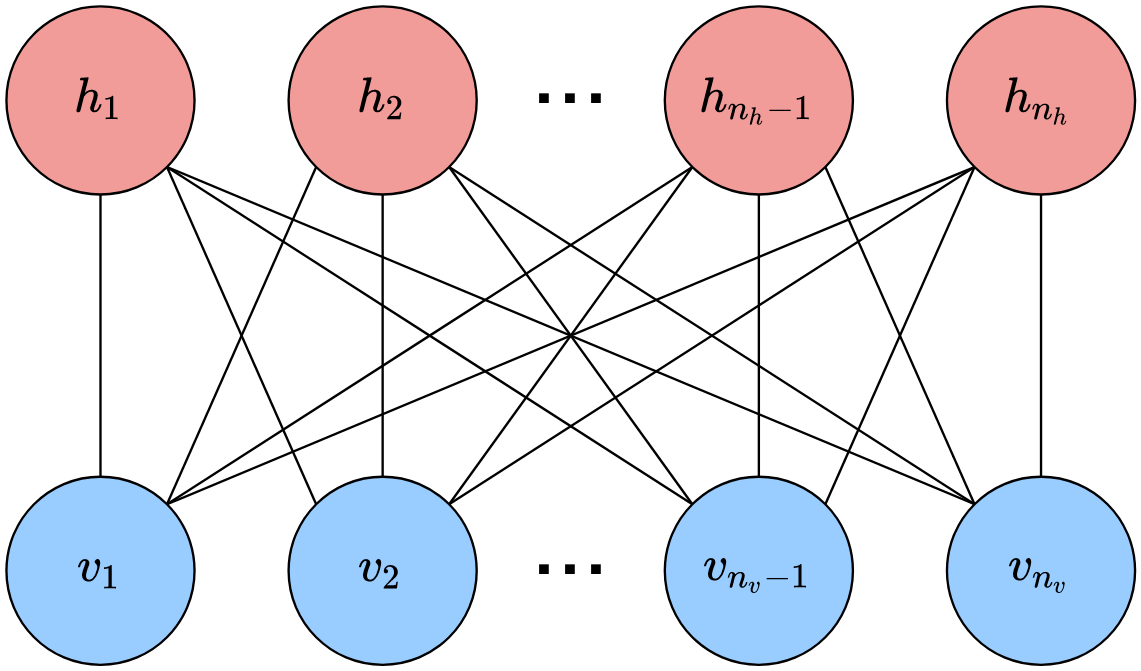
\includegraphics[width=1\linewidth]{rbm_diagram.png}
    \end{center}
    \caption{The structure of a restricted Boltzmann machine with \( n_v \) visible units and \( n_h \) hidden units.}
    \label{fig:rbm_diagram}
\end{figure}

It is termed "restricted" due to the fact that intra-layer connections are not allowed, i.e., visible units are only connected to hidden units, and vice versa.
An example is depicted in \cref{fig:rbm_diagram}.
We also Note that in this case we use RBM to refer to what one might call a Bernoulli RBM, due to the fact that the visible and hidden units are Bernoulli random variables.

The probability to find the system in the configuration \( \{\vec{v},\vec{h}\} \) is given by the Boltzmann distribution (with \( \beta = \frac{1}{k_BT} = 1 \) )
\begin{align}
    p(\vec{v}, \vec{h}) = \frac{1}{Z} e^{-E(\vec{v},\vec{h})}
\end{align}
with intractable~\cite{long_servedio_2010} partition function
\begin{align}
    Z = \sum_{\vec{v},\vec{h}} e^{-E(\vec{v},\vec{h})}
\end{align}

Due to the independence of units in the same layer, the conditional probabilities of the layers are given by~\footnote{Here \( \sigma(x) \) is the logistic sigmoid function and \( \odot \) denotes element-wise multiplication.} (see \cref{app:conditional_probabilities_derivation} for full derivation)
\begin{align}
    p(\vec{h} | \vec{v})
        &= \prod_j \sigma\big( (2\vec{h} - 1) \odot (\vec{b} + \mat{W}^\intercal\vec{v}) \big)_j \\
    p(\vec{v} | \vec{h})
        &= \prod_i \sigma\big( (2\vec{v} - 1) \odot (\vec{a} + \mat{W}\vec{h}) \big)_i
\end{align}

Due to the partition function being intractable, the model able to be solved analytically, thus one must resort to other methods to optimize it such as likelihood maximization.
Rather than maximizing the likelihood function itself, it is common to minimize the negative log-likelihood.
For data distribution \( p_\text{data} \) and parameters \( \theta = (\mat{W}, \vec{a}, \vec{b}) \) the average log-likelihood is given by
\begin{align}
    \ell(\theta) = \sum_{\vec{v}} p_{\text{data}}(\vec{v}) \log \sum_\vec{h} \frac{1}{Z} e^{-E(\vec{v},\vec{h})}
\end{align}
with gradients (see \cref{app:rbm_log_likelihood_derivation} for full derivation)
\begin{align}
    \partial_{w_{ij}} \ell(\theta)
        &= \langle v_i h_j \rangle_{\text{data}} - \langle v_i h_j \rangle_{\text{model}} \\
    \partial_{a_i} \ell(\theta)
        &= \langle v_i \rangle_{\text{data}} - \langle v_i \rangle_{\text{model}} \\
    \partial_{b_j} \ell(\theta)
        &= \langle h_j \rangle_{\text{data}} - \langle h_j \rangle_{\text{model}}
\end{align}
Therefore, the parameters at step \( t \) are given by
\begin{align}
    \mat{W}^{(t)}
        &= \mat{W}^{(t-1)} + \eta(\langle \vec{v} \vec{h}^\intercal \rangle_{\text{data}} - \langle \vec{v} \vec{h}^\intercal \rangle_{\text{model}}) \\
    \vec{a}^{(t)}
        &= \vec{a}^{(t-1)} + \eta(\langle \vec{v} \rangle_{\text{data}} - \langle \vec{v} \rangle_{\text{model}}) \\
    \vec{b}^{(t)}
        &= \vec{b}^{(t-1)} + \eta(\langle \vec{h} \rangle_{\text{data}} - \langle \vec{h} \rangle_{\text{model}})
\end{align}
where \( \eta \) is the learning rate hyperparameter.

Since \( p(\vec{v}) \) can not be sampled directly, it must be sampled using a Markov chain Monte Carlo (MCMC) method.
The way to do so is through Gibbs sampling, which uses the conditional probabilities \( p(\vec{h}|\vec{v}) \) and \( p(\vec{v}|\vec{h}) \).
One starts with a visible vector and then samples the hidden units, followed by sampling the visible units, and so forth until a desired thermalization threshold is reached.
How many steps it requires to reach thermalization is model dependent, and can be estimated by analyzing the autocorrelations of a Markov chain.
The algorithm for Gibbs sampling is given in \cref{alg:Gibbs} and illustrated in \cref{fig:gibbs_sampling_diagram}.
For brevity the algorithm is presented in a vectorized format.

\begin{algorithm}
\caption{Gibbs Sampling}
\begin{algorithmic}[1]
    \Procedure{Gibbs}{$\vec{v},n,\mat{W},\vec{a},\vec{b}$}
        \State $n_v \gets$ length$(\vec{a})$
        \State $n_h \gets$ length$(\vec{b})$
        \For{$k$ in 1 to $n$}
            \State $\vec{r} \sim$ Uniform$(0, 1, n_h)$
            \State $\vec{h} \gets \vec{r} < \sigma(\vec{b} + \mat{W}^\intercal\vec{v})$
                \Comment $\sigma, <$ applied element-wise
            \State $\vec{r} \sim$ Uniform$(0, 1, n_v)$
            \State $\vec{v} \gets \vec{r} < \sigma(\vec{a} + \mat{W}\vec{h})$
                \Comment $\sigma, <$ applied element-wise
        \EndFor
        \State \Return $\vec{v}$
    \EndProcedure
\end{algorithmic}
\label{alg:Gibbs}
\end{algorithm}
The Uniform$(a, b, n)$ function in \cref{alg:Gibbs} produces a length \( n \) vector of uniform i.i.d. random variables on the interval $[a, b)$.

\begin{figure}
    \begin{center}
        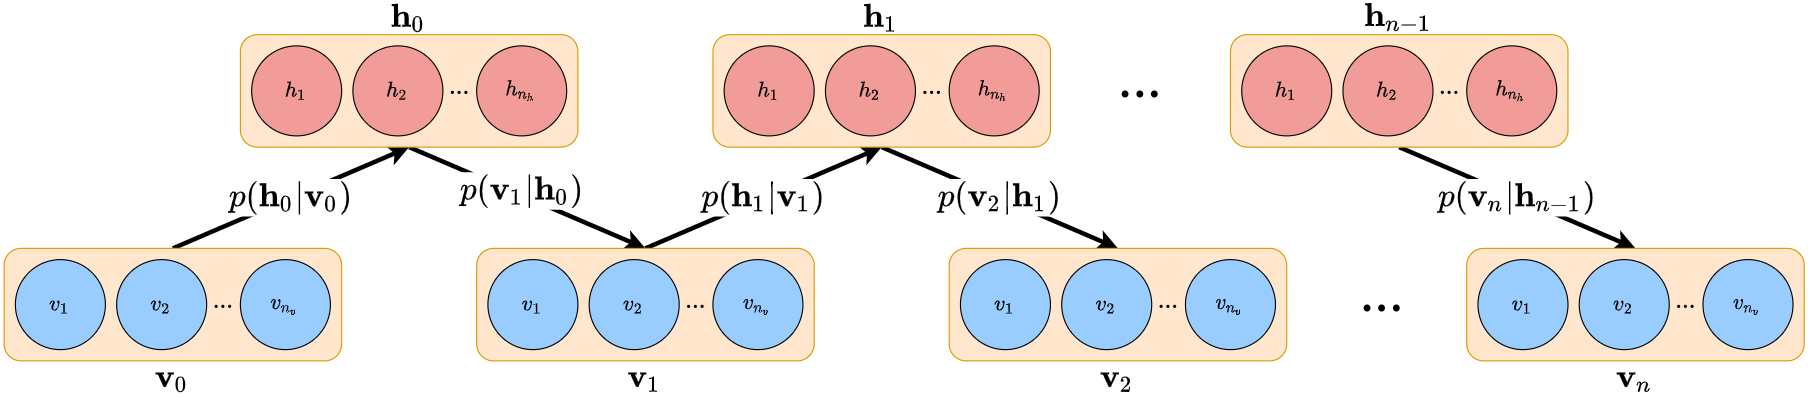
\includegraphics[width=1\linewidth]{gibbs_sampling_diagram.png}
    \end{center}
    \caption{Illustration of the Gibbs sampling procedure.}
    \label{fig:gibbs_sampling_diagram}
\end{figure}

The standard procedure for training an RBM is called \( n \)-step contrastive divergence (CD-\( n \)), with \( n \) often taken as 1 in practice.
The algorithm is detailed in \cref{alg:CDn}, where one can see that \( n \) corresponds to how many Gibbs sampling steps are between the positive and negative phase gradient estimates.
Applying the algorithm to a mini-batch is essentially the same except except that one divides the learning rate by the size of the mini-batch to get a mini-batch averaged gradient estimate.

\begin{algorithm}
    \caption{$n$-Step Contrastive Divergence (CD-$n$)}
\begin{algorithmic}[1]
    \Procedure{CD}{$\vec{v}_+,n,\mat{W},\vec{a},\vec{b},\eta$}
        \Comment $\vec{v}_+$ is a training example
        \State $\vec{h}_+ \gets \sigma(\vec{b} + \mat{W}^\intercal\vec{v}_+)$
            \Comment $\sigma$ applied element-wise
        \State $\vec{v}_- \gets$ Gibbs$(\vec{v}_+,n,\mat{W},\vec{a},\vec{b})$
        \State $\vec{h}_- \gets \sigma(\vec{b} + \mat{W}^\intercal\vec{v}_-)$
            \Comment $\sigma$ applied element-wise
        \State $\mat{W} \gets \mat{W} + \eta(\vec{v}_+ \vec{h}_+^\intercal - \vec{v}_- \vec{h}_-^\intercal)$
        \State $\vec{a} \gets \vec{a} + \eta(\vec{v}_+ - \vec{v}_-)$
        \State $\vec{b} \gets \vec{b} + \eta(\vec{h}_+ - \vec{h}_-)$
        \State \Return $\mat{W}, \vec{a}, \vec{b}$
    \EndProcedure
\end{algorithmic}
\label{alg:CDn}
\end{algorithm}


%\section{Application}

%\section{Results}
%In this section we will compare four different RBM models, denoted as:
%\begin{itemize}
    %\item (B): baseline model.
    %\item (V): using volatility indicators.
    %\item (X): using a transformed feature space.
    %\item (XV): using a transformed feature space and volatility indicators.
%\end{itemize}

%\begin{table}[ht]
    %\centering
    %\begin{adjustbox}{max width=\textwidth}
        %\input{../tables/rbm/correlation_coefficients.tbl}
    %\end{adjustbox}
    %\caption{Correlation coefficients of the data vs. samples generated by the RBM models. The RBM numbers are shown in the format average \(\pm\) 1 standard deviation from an ensemble of size 100.}
    %\label{tbl:rbm_correlation_coefficients}
%\end{table}

%\begin{table}[ht]
    %\centering
    %\begin{adjustbox}{max width=\textwidth}
        %\input{../tables/rbm/qq_rmses.tbl}
    %\end{adjustbox}
    %\caption{QQ root mean squared errors of the RBM models. All numbers are shown in the format average \(\pm\) 1 standard deviation from an ensemble of size 100.}
    %\label{tbl:rbm_qq_rmse}
%\end{table}

%\begin{table}[ht]
    %\centering
    %\begin{adjustbox}{max width=\textwidth}
        %\input{../tables/rbm/volatilities.tbl}
    %\end{adjustbox}
    %\caption{Historical volatilities of the data vs. samples generated by the RBM models. All numbers are shown in the format average \(\pm\) 1 standard deviation from an ensemble of size 100.}
    %\label{tbl:rbm_volatilities}
%\end{table}

%\begin{table}[ht]
    %\centering
    %\begin{adjustbox}{max width=\textwidth}
        %\input{../tables/rbm/conditional_volatilities.tbl}
    %\end{adjustbox}
    %\caption{Conditional historical volatilities of the data vs. samples generated by the RBM models. All numbers are shown in the format average \(\pm\) 1 standard deviation from an ensemble of size 100.}
    %\label{tbl:rbm_conditional_volatilities}
%\end{table}

%\begin{table}[ht]
    %\centering
    %\begin{adjustbox}{max width=\textwidth}
        %\input{../tables/rbm/autocorrelation_times.tbl}
    %\end{adjustbox}
    %\caption{Integrated autocorrelation times of the RBM models.}
    %\label{tbl:rbm_ac_times}
%\end{table}

%\begin{table}[ht]
    %\centering
    %\begin{adjustbox}{max width=\textwidth}
        %\input{../tables/rbm/tails.tbl}
    %\end{adjustbox}
    %\caption{Lower and upper tails, i.e., 1st and 99th percentiles, of the data vs. samples generated by the RBM models. All numbers are shown in the format average \(\pm\) 1 standard deviation from an ensemble of size 100.}
    %\label{tbl:rbm_tails}
%\end{table}

%\begin{figure}[ht]
    %\begin{center}
        %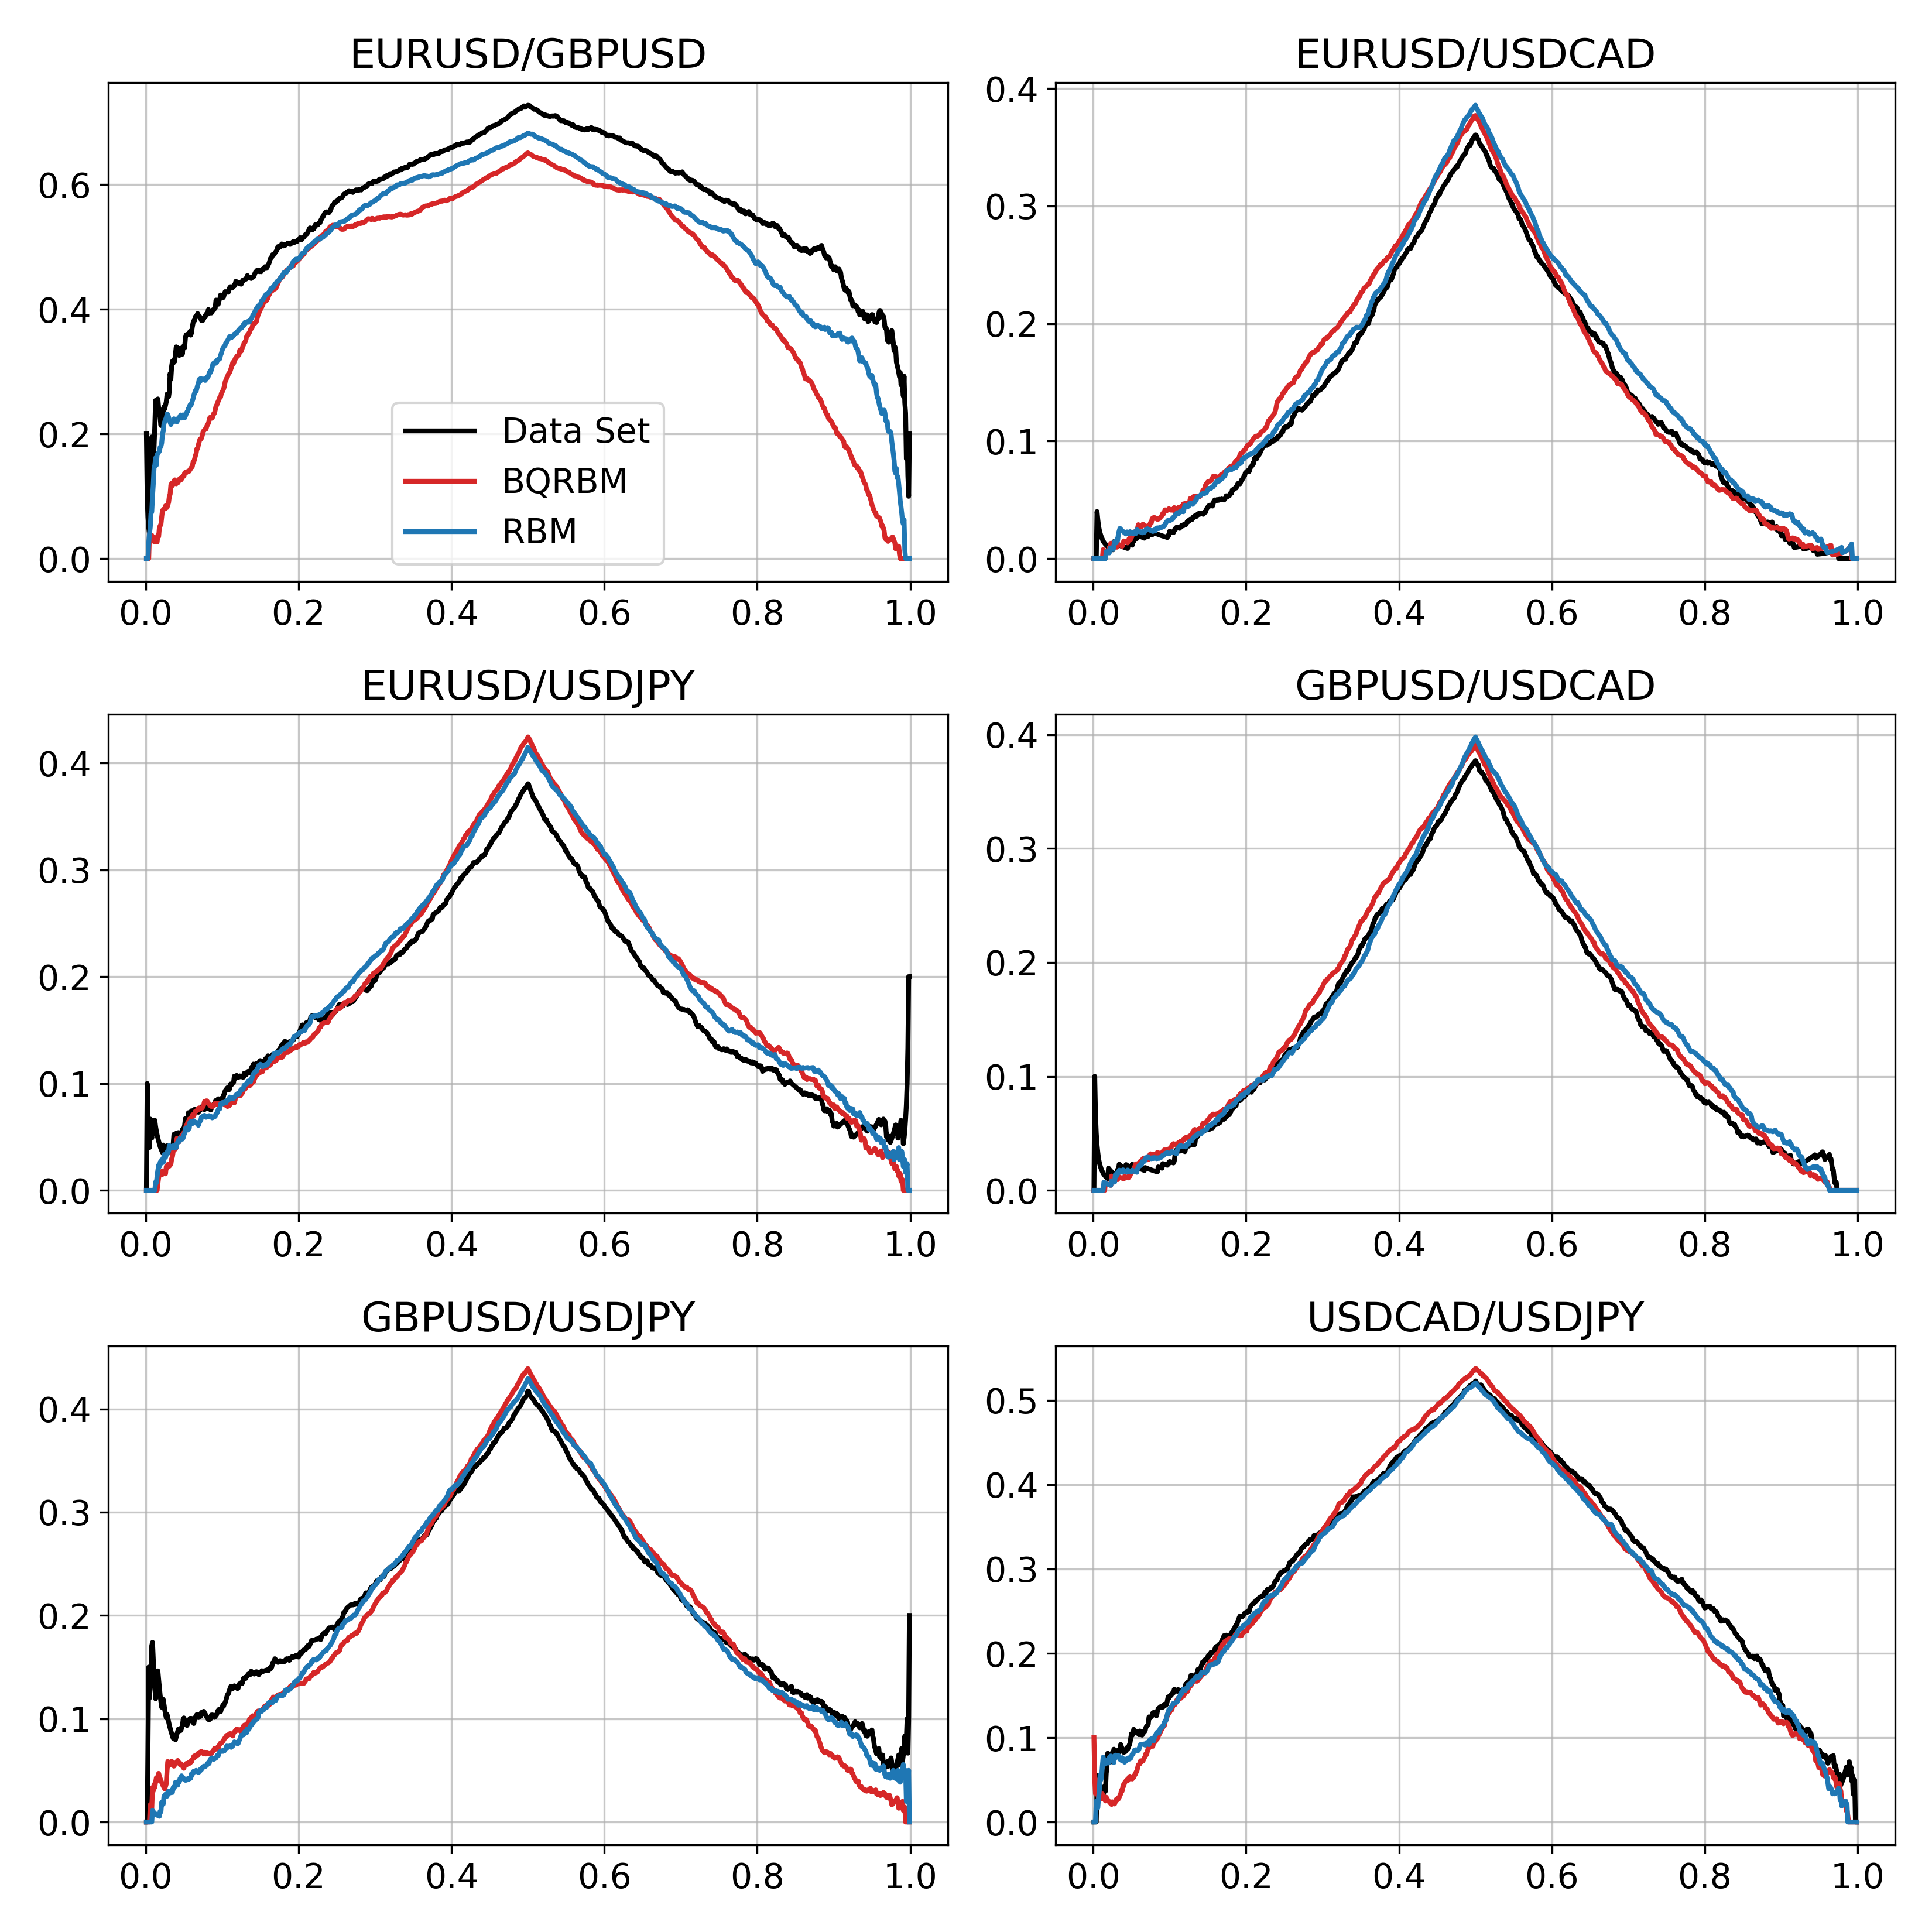
\includegraphics[width=1\linewidth]{rbm/tail_concentrations.png}
    %\end{center}
    %\caption{Tail concentration functions of the data vs. samples generated by the RBM models.}
    %\label{fig:rbm_tail_concentrations}
%\end{figure}

%\begin{figure}[ht]
    %\begin{center}
        %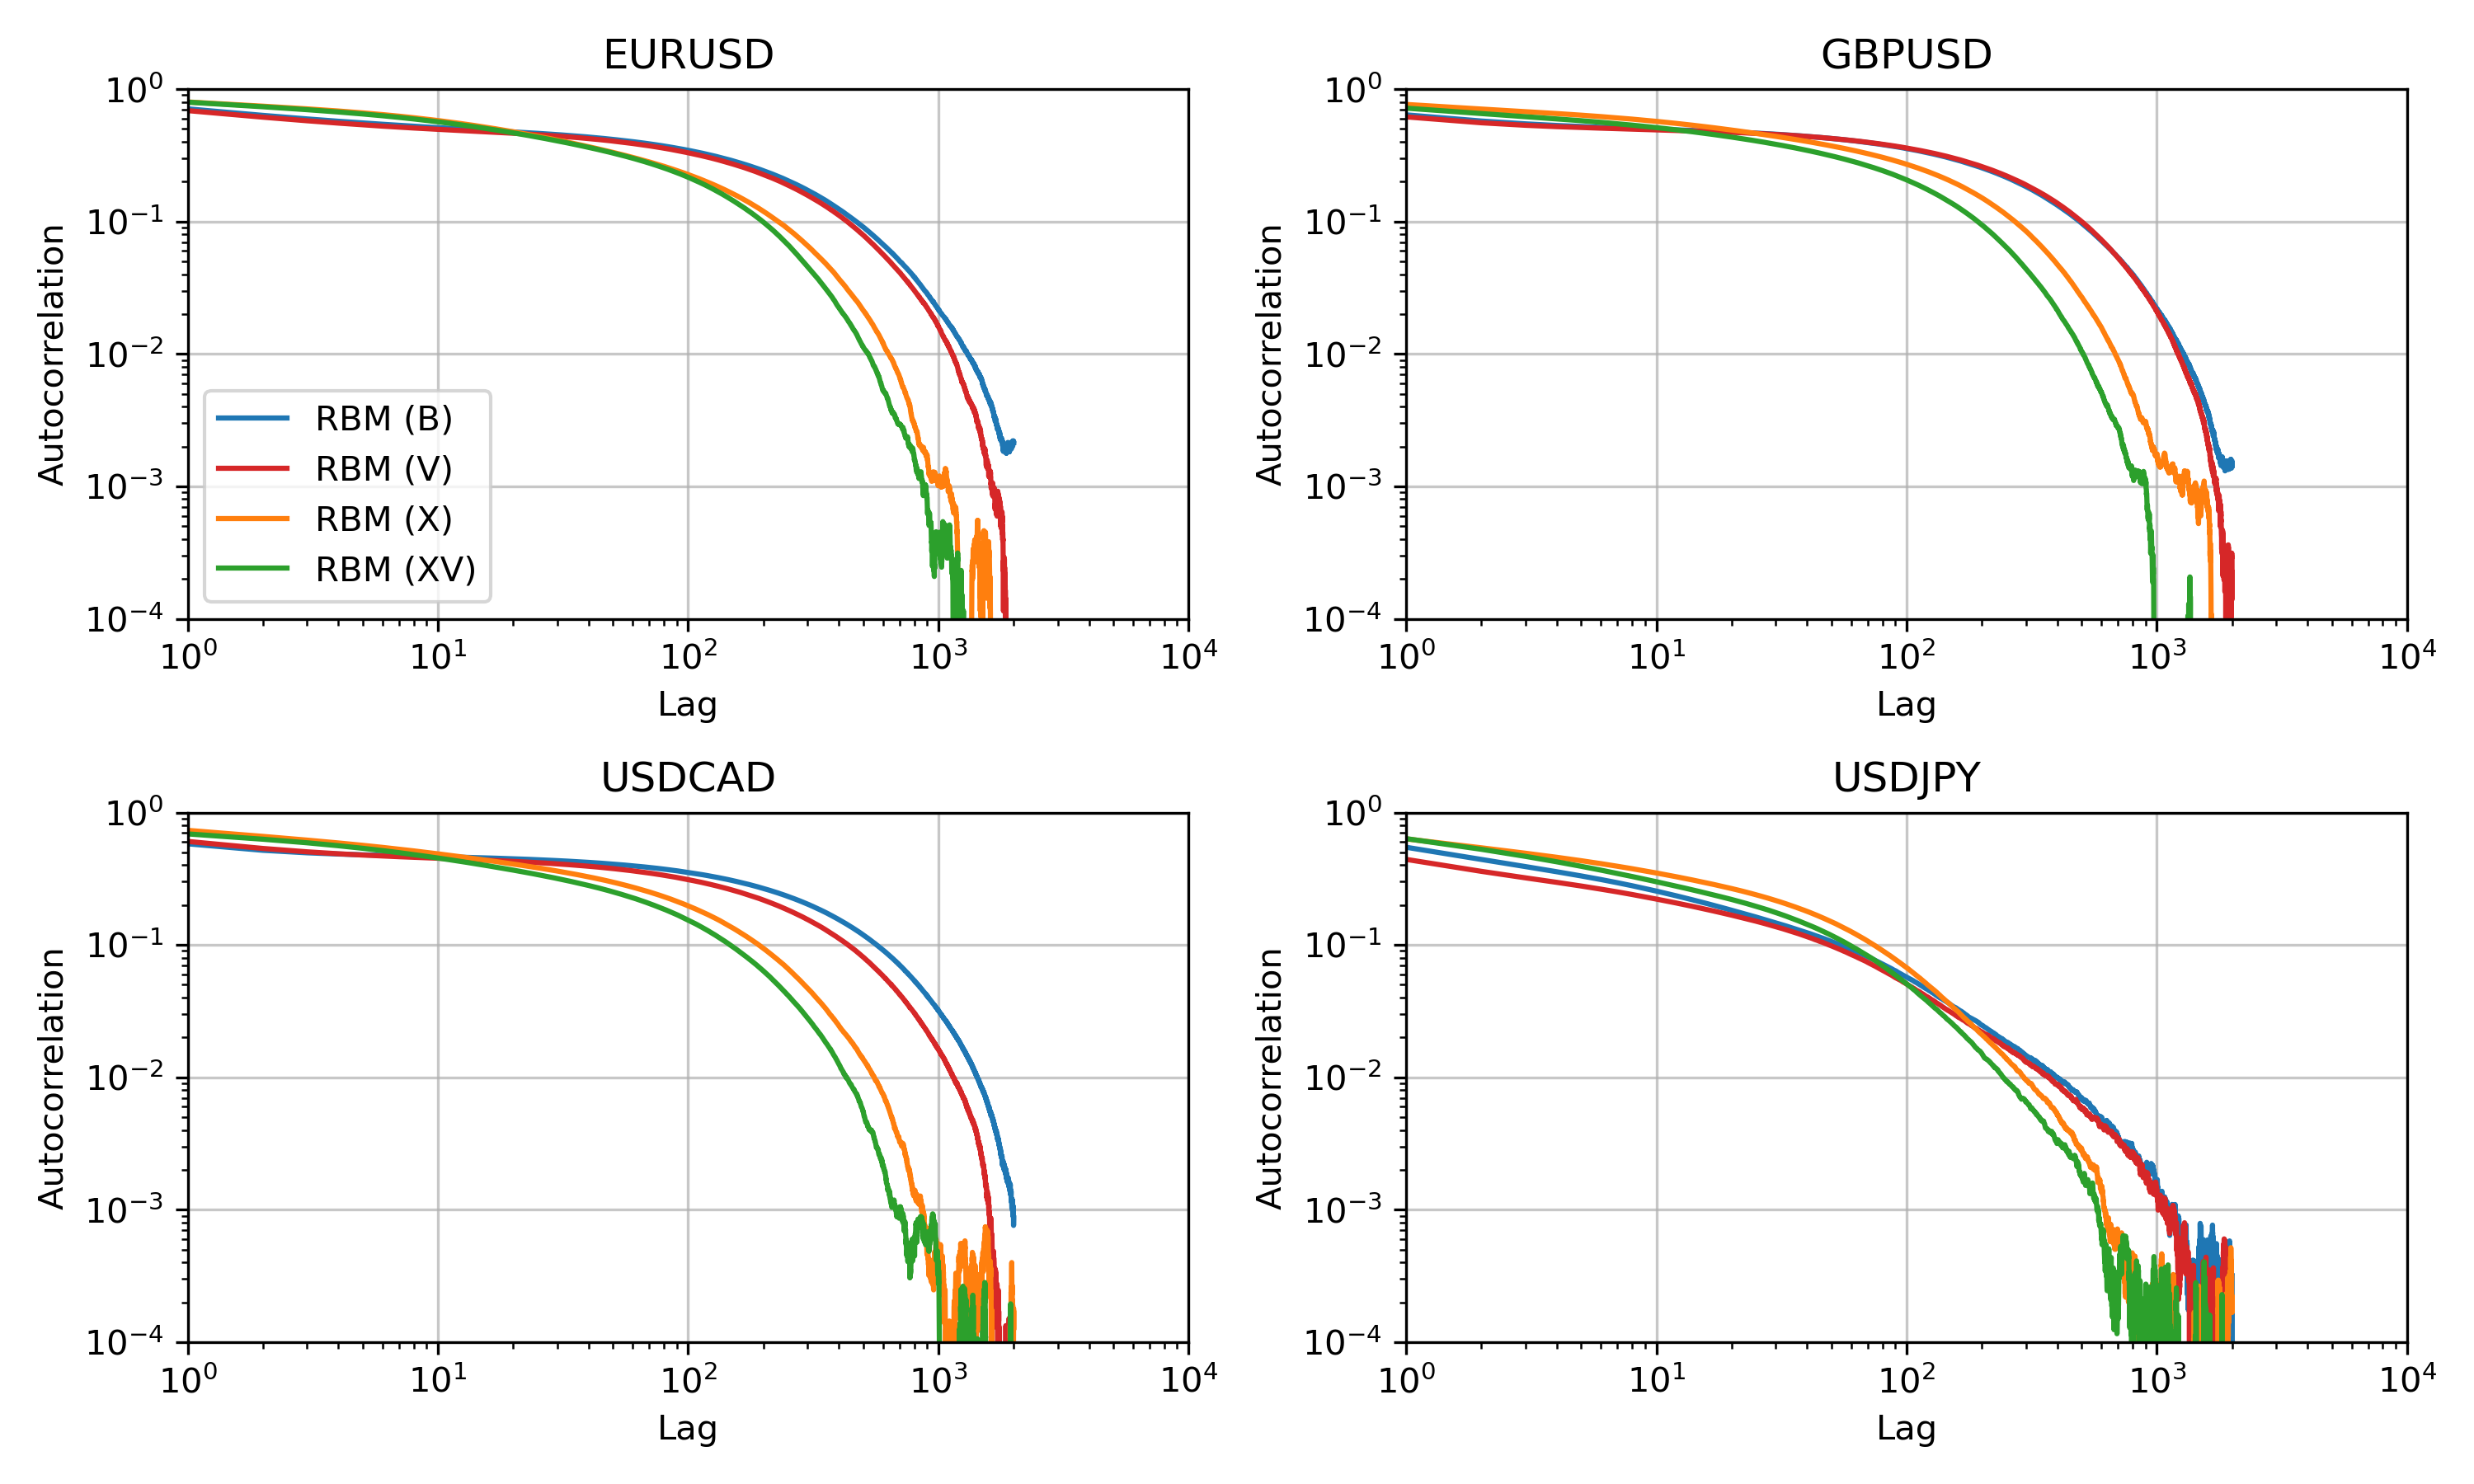
\includegraphics[width=1\linewidth]{rbm/autocorrelation_functions.png}
    %\end{center}
    %\caption{Autocorrelation functions of the RBM models. Function values are computed from Gibbs sample chains of length \( 10^8 \).}
    %\label{fig:rbm_autocorrelation_functions}
%\end{figure}

%\begin{figure}[ht]
    %\begin{center}
        %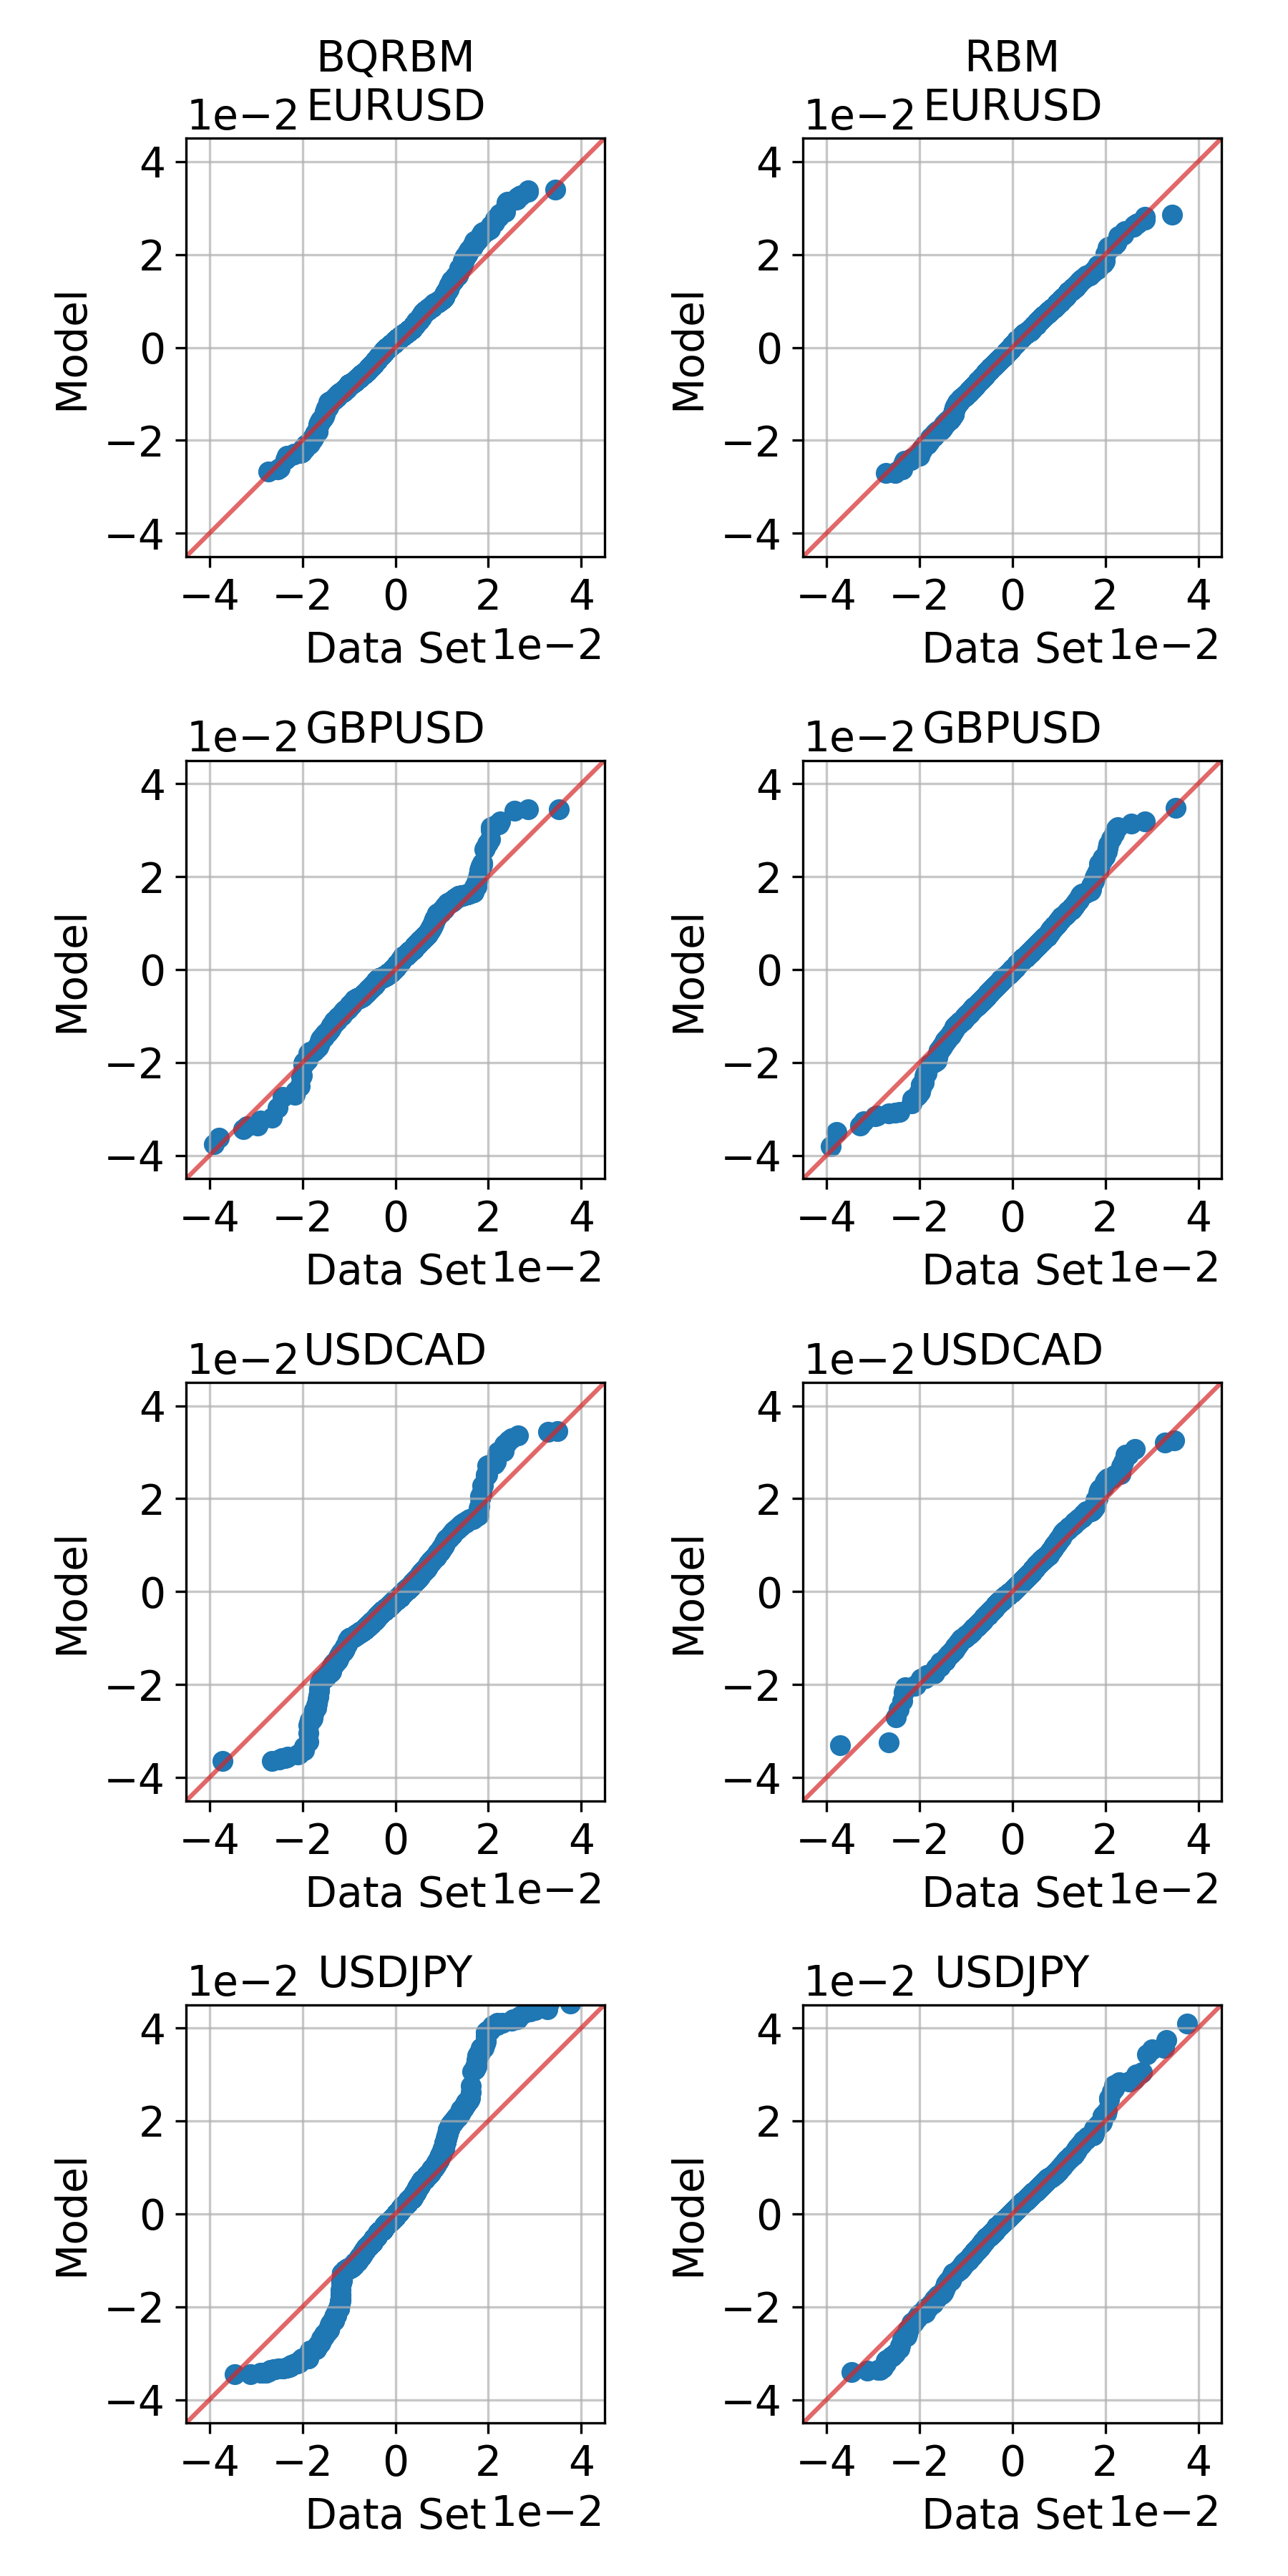
\includegraphics[width=1\linewidth]{rbm/qq.png}
    %\end{center}
    %\caption{QQ plots of the RBM models.}
    %\label{fig:rbm_qq_plots}
%\end{figure}
